\documentclass[xetex]{beamer}
\usepackage{fontspec}

\title{Automatisk upptäckt av strukturer för binära nätverksprotokoll}
\author{Fredrik Appelros \& Carl Ekerot}
\date

% Introducera problemet - applikationer
% Tidigare försök
% Kort om vårt angreppssätt
% Hitta pakettyper (2 delar)
% Klustring
% Förfining av typindelning
% Fältanalys (bygger på bytefördelningar)
% Olika fälttyper
% Tillståndsdiagram
% Resultat - jämförelse mellan definition och inferens
% Begränsningar

\begin{document}
    \frame{\titlepage}
    
    % Introduktion
    \begin{frame}
        \frametitle{Binära nätveksprotokoll}
        Beskriv binära nätverksprotokoll
    \end{frame}
    \begin{frame}
        \frametitle{Slutna protokoll}
        Beskriv hur det kan finnas behov av att hitta struktur i
        ospecifierade binära nätveksprotokoll
    \end{frame}
    \begin{frame}
        \frametitle{Tidigare försök}
        Berätta om Discoverer, exekveringstillstånds-approachen osv.
    \end{frame}

    % Vår approach
    \begin{frame}
        \frametitle{Vårt angreppssätt}
        Kort om hur vi tillämpar metoder från statistisk analys så
        som t.ex. klustring och diverse heurestiker.
    \end{frame}
    
    % Klustring
    \begin{frame}
        \frametitle{Hitta meddelandetyper}
        Beskriv hur vi delar upp sökandet efter typer i två pass
    \end{frame}
    \begin{frame}
        \frametitle{Hitta meddelandetyper -- Klustring}
        Hur vi använder OPTICS för att hitta gruppering av meddelanden som
        liknar varandra enligt våra features
    \end{frame}
    \begin{frame}
        \frametitle{Hitta meddelandetyper -- Förfining}
        Type distinguisher clustering
    \end{frame}

    % Fält
    \begin{frame}
        \frametitle{Protokollens fält}
        Beskriv vad fält är, hur de brukar vara alignade, vilka olika typer
        som vi anser det finnas. Berätta om bytevärdesdistribution
    \end{frame}
    \begin{frame}
        \frametitle{Konstanta fält}
        \begin{columns}[t]
            \begin{column}[T]{6cm}
                Hur vi hittar konstanta fält
            \end{column}
            \begin{column}[T]{6cm}
                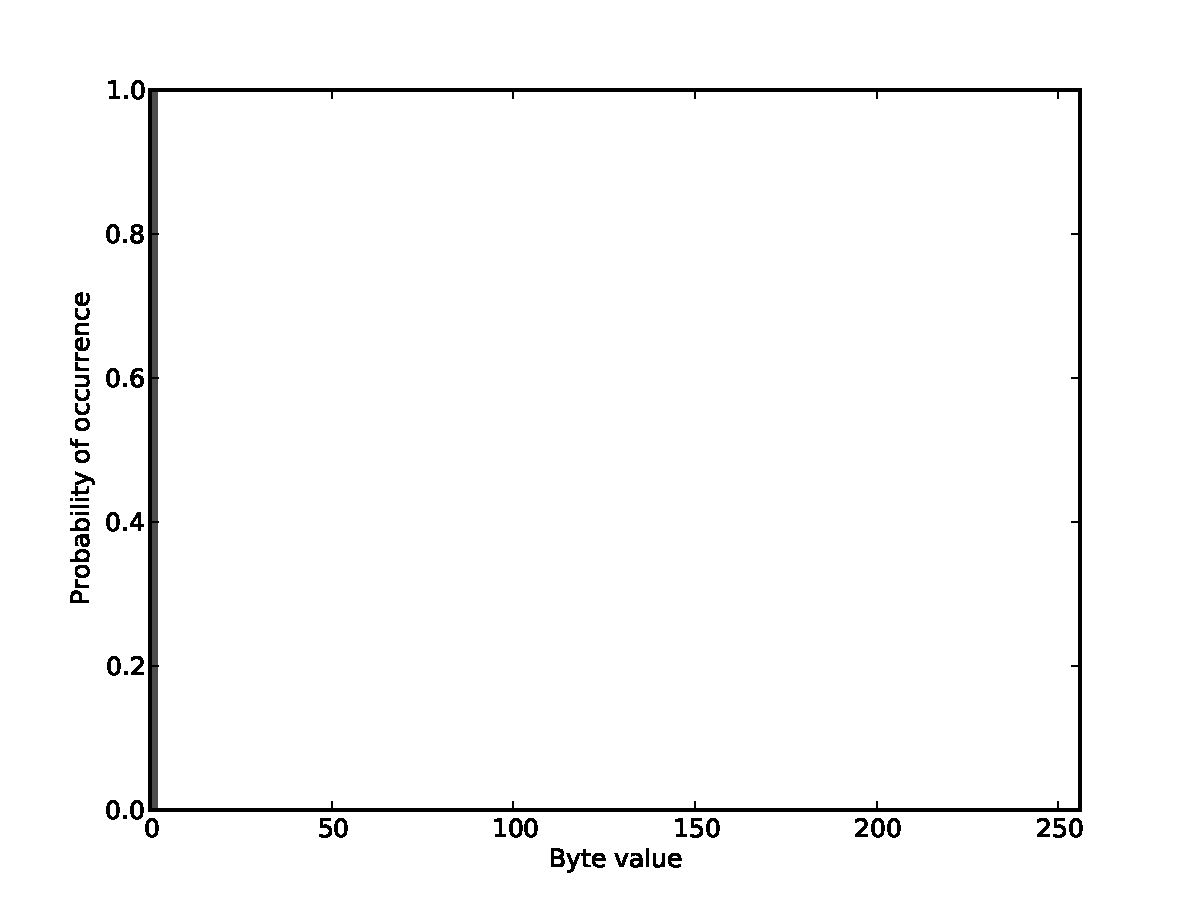
\includegraphics[height=5cm]{img/const_one.pdf}
            \end{column}
        \end{columns}
    \end{frame}
    \begin{frame}
        \frametitle{Flaggfält}
        \begin{columns}[t]
            \begin{column}[T]{6cm}
                Hur vi hittar flaggfält
            \end{column}
            \begin{column}[T]{6cm}
                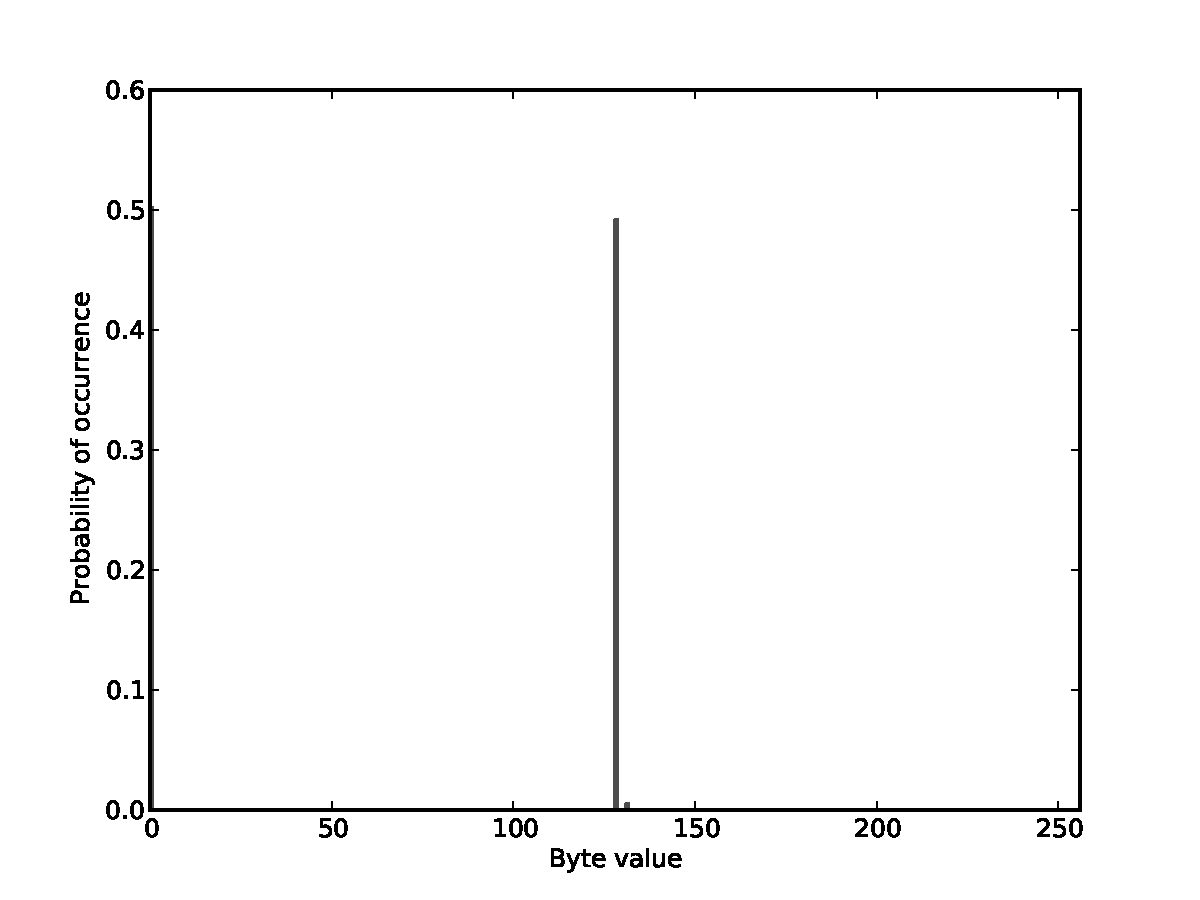
\includegraphics[height=5cm]{img/flag.pdf}
            \end{column}
        \end{columns}
    \end{frame}
    \begin{frame}
        \frametitle{Uniformt fördelade fält}
        \begin{columns}[t]
            \begin{column}[T]{6cm}
                Hur vi hittar uniformt fördelade fält
            \end{column}
            \begin{column}[T]{6cm}
                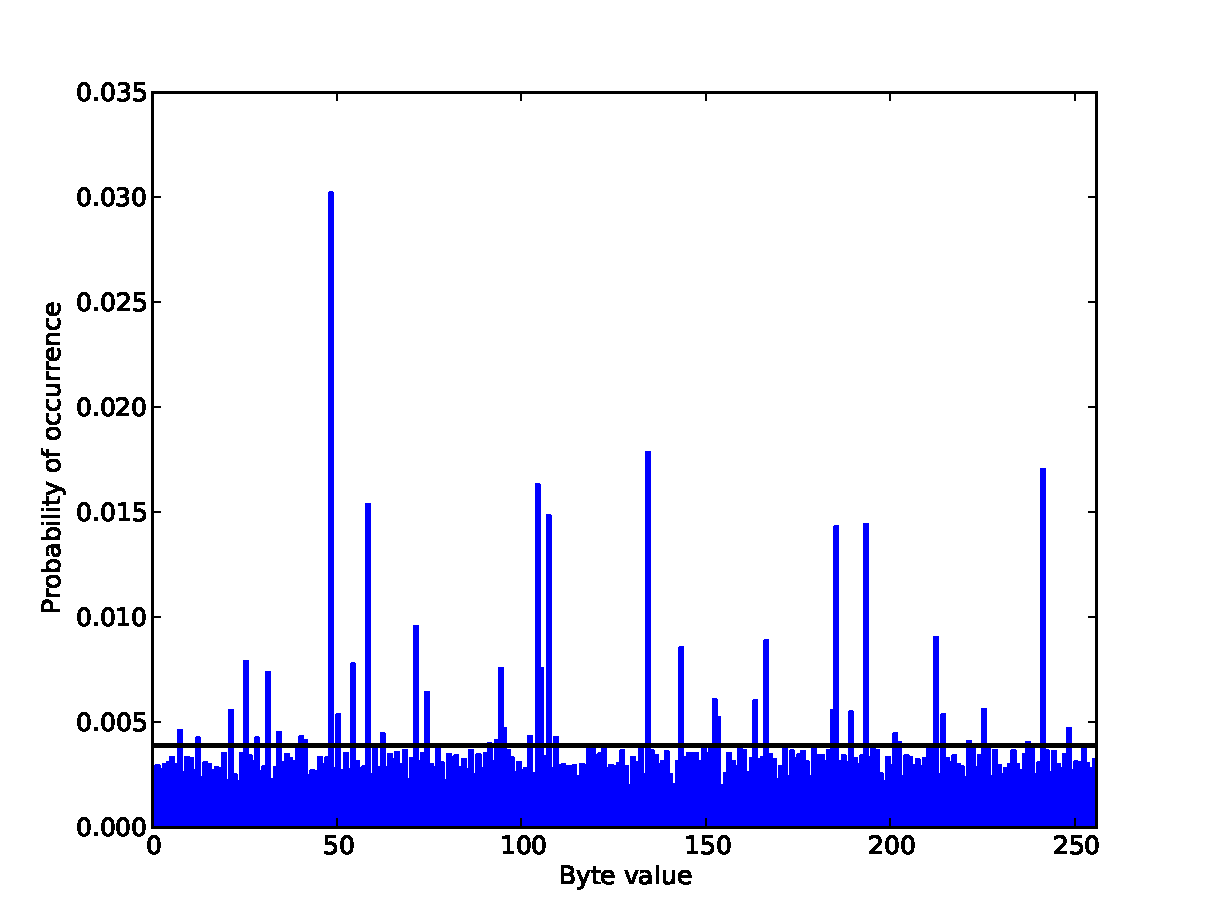
\includegraphics[height=5cm]{img/uniform.pdf}
            \end{column}
        \end{columns}
    \end{frame}
    \begin{frame}
        \frametitle{Nummerfält}
        \begin{columns}[t]
            \begin{column}[T]{6cm}
                Hur vi hittar nummerfält
            \end{column}
            \begin{column}[T]{6cm}
                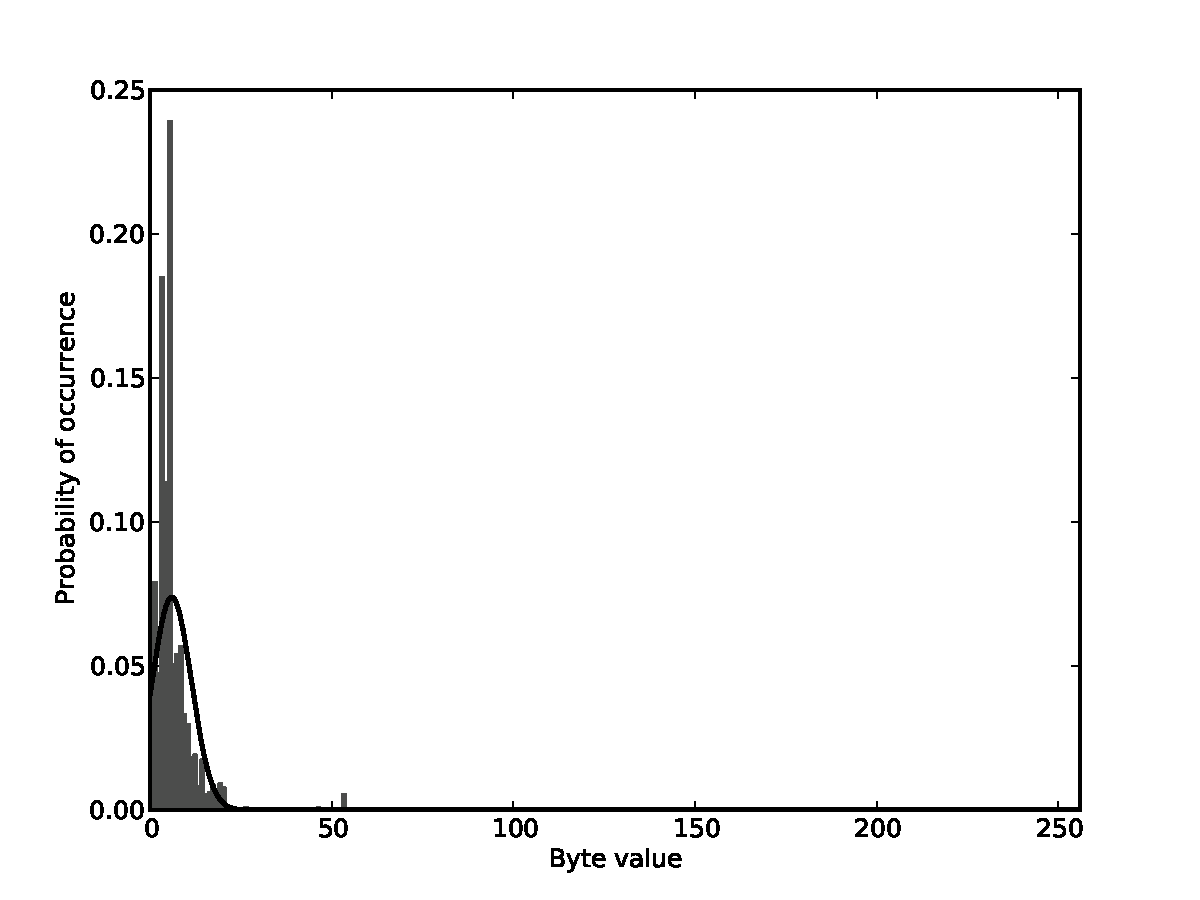
\includegraphics[height=5cm]{img/number.pdf}
            \end{column}
        \end{columns}
    \end{frame}
    \begin{frame}
        \frametitle{Inkrementella fält}
        Hur vi hittar inkrementella fält
    \end{frame}
    \begin{frame}
        \frametitle{Längdfält}
        \begin{columns}[t]
            \begin{column}[T]{6cm}
                Hur vi hittar längdfält
            \end{column}
            \begin{column}[T]{6cm}
                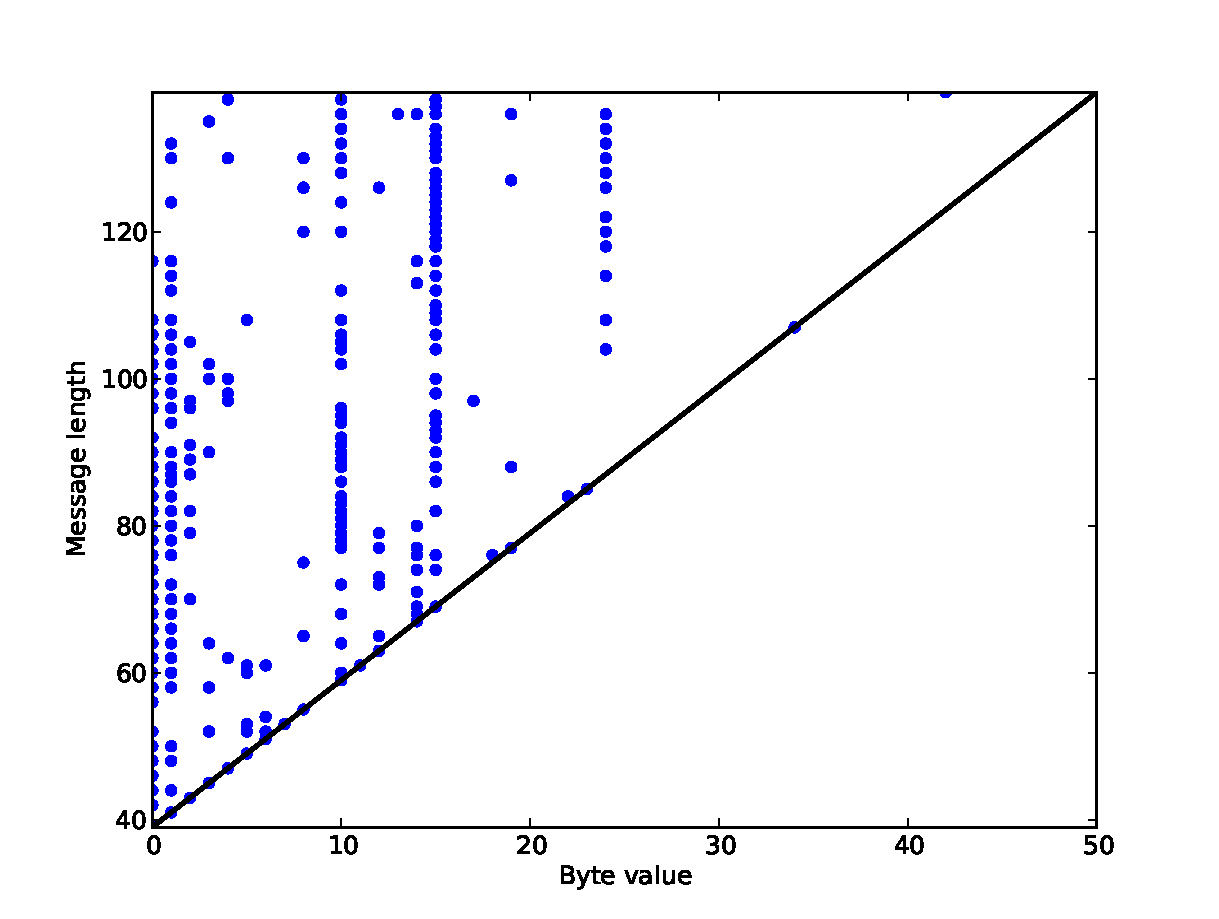
\includegraphics[height=5cm]{img/length.pdf}
            \end{column}
        \end{columns}
    \end{frame}

    % Tillstånd
    \begin{frame}
        \frametitle{Protokolls tillstånd}
        Beskriv hur många protokoll har ett antal tillstånd och hur vi
        hittar dem. Beskriv varför det inte alltid är rimligt att hitta
        alla möjliga tillstånd.
    \end{frame}

    % Resultat
    \begin{frame}
        \frametitle{Resultat}
        Visa resultat och prestanda
    \end{frame}
    \begin{frame}
        \frametitle{Demo?}
        Demonstrera?
    \end{frame}

    % Begränsningar
    \begin{frame}
        \frametitle{Begränsningar}
        Berätta vad som krävs för att kunna göra en bra analys
    \end{frame}

\end{document}
